\documentclass[]{spie}  %>>> use for US letter paper
%\documentclass[a4paper]{spie}  %>>> use this instead for A4 paper
%%\documentclass[nocompress]{spie}  %>>> to avoid compression of citations

\renewcommand{\baselinestretch}{1.0} % Change to 1.65 for double spacing

\usepackage{algorithm}
\usepackage{algorithmic}
\usepackage{comment}
\usepackage{color}
\usepackage{tabularray}
\definecolor{Silver}{rgb}{0.752,0.752,0.752}
\definecolor{Mercury}{rgb}{0.901,0.901,0.901}
\usepackage{amsmath,amsfonts,amssymb}
\usepackage{graphicx}
\usepackage{multirow}
\usepackage{colortbl}
\usepackage{pgfplots}
\usepackage{tikz}
\pgfplotsset{compat=1.17}
\pgfplotsset{compat=1.3}
\usepackage{booktabs}
\usepackage{hhline}
\usepackage{float}
\usepackage[table,xcdraw]{xcolor} % Needed for coloring tables
\usepackage{caption}
\usepackage{tabularray}





\definecolor{Gray1}{gray}{0.9}
\definecolor{Gray2}{gray}{0.8}
\definecolor{ppink}{HTML}{ec81fc}
\definecolor{oorange}{HTML}{eda477}
\definecolor{bbrown}{HTML}{826441}
\definecolor{peridot}{rgb}{0.9, 0.89, 0.0}
\definecolor{richlavender}{rgb}{0.67, 0.38, 0.8}
\definecolor{Silver}{rgb}{0.752,0.752,0.752}

\definecolor{forestgreen}{rgb}{0.0, 0.27, 0.13}
\definecolor{darkcandyapplered}{rgb}{0.64, 0.0, 0.0}
\definecolor{paleplum}{rgb}{0.8, 0.6, 0.8}
\definecolor{pastelorange}{rgb}{1.0, 0.7, 0.28}

\definecolor{yellow-green}{rgb}{0.6, 0.8, 0.2}
\definecolor{wenge}{rgb}{0.39, 0.33, 0.32}
\definecolor{corn}{rgb}{0.98, 0.93, 0.36}
\definecolor{darkpowderblue}{rgb}{0.0, 0.2, 0.6}
\definecolor{dimgray}{rgb}{0.41, 0.41, 0.41}
\usepackage{graphicx}
\usepackage[colorlinks=true, allcolors=blue]{hyperref}

\title{Scheduling Algorithms on Heterogeneous Architectures for Efficient Vision Systems}

\author[]{Teymoor Ali. }
\author[a,b]{George Paul. }
\author[a]{Deepayan Bhowmik.}
\author[b]{Robert Nicol.}
\affil[a]{Newcastle University, 1 Science Square, Newcastle upon Tyne, U.K}
\affil[b]{STMicroelectronics, 1 Tanfield, Inverleith Row, Edinburgh, U.K}

\authorinfo{Further author information: (Send correspondence to T. Ali)\\T. Ali: E-mail: Teymoor.A@outlook.com, \\  G.P E-mail: George.Paul@newcastle.ac.uk.}

% Option to view page numbers
\pagestyle{empty} % change to \pagestyle{plain} for page numbers   
\setcounter{page}{301} % Set start page numbering at e.g. 301
 
\begin{document} 
\maketitle

\begin{abstract}
Deep Neural Network (DNN) algorithms have become ubiquitous within the vision domain, encompassing various tasks, including object detection, segmentation, and classification. However, executing complex DNN algorithms on real-time vision systems demands better energy efficiency, runtime, and accuracy requirements. The growing demand for image processing algorithms on systems with resource and energy constraints requires architectures that perform tasks efficiently. Traditionally, embedded imaging designs often involve implementing image processing algorithms on homogeneous architectures, which have hardware limitations. This has led to innovative computing architectures, leveraging heterogeneity that combines CPUs, GPUs, FPGAs, and other accelerators into a single processing fabric. This design choice allows applications to utilise the most efficient architecture for a given algorithm.

However, scheduling and partitioning algorithms remain arduous, particularly when distributing operations among accelerators with different computing paradigms. This challenge requires a balance, considering important factors such as computational power, memory bandwidth, and communication overhead. In addition, scheduling tasks involves determining the order in which tasks are executed while considering factors such as task dependencies, resource availability, and synchronisation. Current state-of-the-art deep learning libraries are primarily designed to target single architectures for model deployment and often lack mechanisms to intelligently partition an algorithm's sub-operations across the most suitable processor. This paper presents a scheduler targeting heterogeneous vision systems, carefully fine-grain partitions and maps sub-operations of widely used convolutional neural networks and image processing algorithms. The results show that the heterogeneous platform is $1.11\times$ \& $1.08\times$ more efficient in kernel runtime and energy consumption than their best performing discrete hardware counterparts, GPU and FPGA. The experiments reveal that partitioning algorithms based on their runtime and energy properties on a given accelerator and optimally scheduled perform better in energy and runtime efficiency than their best-performing homogeneous components executing the complete algorithm.
\end{abstract}

% Include a list of keywords after the abstract 
\keywords{Heterogeneous Computing, Computer Vision, FPGA-GPU, Heterogenous Scheduler}


\section{INTRODUCTION}
\label{sec:intro}
Vision systems have increasingly become pervasive in many application domains, particularly those utilising deep learning (DL) algorithms such as Satellites \cite{10.1145/2491956.2462176}, Autonomous Vehicles \cite{kuutti2020survey}, and Remote Sensing \cite{YUAN2020111716}. However, many of these systems face low-SWaP (Size, Weight, and Power) constraints, adding further complexity and limiting available resources. Traditionally, most hardware architectures are composed of homogeneous compute units coupled with fixed memory hierarchies, such as Central Processing Units (CPUs) or Graphics Processing Units (GPUs). While these architectures compute specific algorithms efficiently, in some cases, performance is traded off for flexibility, leading to poorer execution for operations that do not fit the design. This rigidity becomes particularly problematic when deploying deep learning models with diverse computational needs. The diverse operators within deep learning and image processing workloads, ranging from convolutional layers to recurrent networks, often exhibit varying levels of parallelism and memory access patterns.

Heterogeneous architectures have been shown as a potential path forward to keep up with the rising demand for better performance. This hardware paradigm integrates various compute accelerators to form a single compute fabric, sharing resources whilst leveraging their unique processing characteristics. Computer vision algorithms comprise various image processing and deep learning algorithms, forming a pipeline. GPUs, with their massively parallel architecture consisting of thousands of cores, streaming multiprocessors (SMs), and single instruction multiple data (SIMD) units, excel at accelerating pixel-level computations. Their specialised hardware, such as texture units for efficient image filtering and high-bandwidth memory interfaces for fast data access, enables fast execution of pixel processing streams. 

In addition, FPGAs bring their own unique advantages for imaging tasks due to their inherent flexibility and configurable architecture. Unlike fixed-function processors, FPGAs offer the capability to tailor specific image processing algorithms through hardware-level customisation, leveraging programmable logic blocks, custom memory hierarchy, and digital signal processing (DSP) slices. This level of customisation enables the development of highly optimised image processing pipelines finely tuned to specific requirements. Furthermore, FPGAs employ a versatile routing architecture that can be configured to manage dataflow between operations efficiently. This fine-grained control over routing allows data to be directed through the configurable logic fabric with minimal latency. This customisation capability allows for low-latency, real-time processing of image streams. Neural Processing Units often incorporate specialised hardware units, such as systolic arrays or matrix multiplication engines, optimised for the core mathematical operations found in deep neural networks.

Furthermore, as deep neural networks increase in architectural complexity and model size, they demand significant memory resources to store their weights, posing challenges for implementation on resource—and energy-constrained platforms. Despite these challenges, true heterogeneous computing offers a pathway to developing runtime and power-efficient designs. By exploiting architectures with sufficient resources and processing capabilities, it is possible to achieve high-performance computation while adhering to the constraints of resource-limited environments.

Deep learning frameworks such as TensorFlow\cite{tensorflow2015} and PyTorch\cite{Pytorch} provide high-level APIs and abstractions to simplify model development and deployment. These frameworks utilise graph-based intermediate representations (IR) like XLA or TorchScript to enable optimisations and portability across different hardware platforms. Machine learning compilers like TVM\cite{chen2018} or MLIR\cite{mlir} further optimise these IRs for specific targets, leveraging techniques such as operator fusion, memory layout optimisation, and kernel specialisation. However, the current tools often revolve around a single backend, such as CUDA for GPUs. While this simplifies development for specific hardware, it limits the ability to exploit the heterogeneity. Consequently, limiting further hardware and image domain-specific optimisations\cite{ali2023domain}.


In this paper, we propose a scheduler that partitions computer vision pipelines and their sub-algorithms into suitable accelerators, optimising performance and energy efficiency. Subgraphs are generated from PyTorch for each selected pipeline, allowing distinct segments of the algorithms to be independently executed on various accelerators, thus leveraging the strengths of heterogeneous systems. We evaluate the performance of these partitioned pipelines and compare them to their discrete accelerator counterparts, analysing key metrics such as inference time, energy consumption, and accuracy. Additionally, the scheduler's performance is benchmarked against other ML compilers, such as TVM. The feasibility and benefits of this approach offer key insights into optimal deployment strategies for computer vision pipelines on heterogeneous hardware platforms.

% Convolutional Neural Networks (CNNs)  are prevalent in various domains, including object detection\cite{zhao2012flip}, image classification\cite{rawat2017deep}, and image segmentation\cite{minaee2021image}. These image processing algorithms are generally designed and implemented on GPUs, which feature thousands of compute cores coupled with high-bandwidth memory. This configuration enables efficient execution of Single Instruction, Multiple Data (SIMD) operations, making GPUs ideal for parallel processing of extensive data sets. However, the execution of algorithms on GPUs involves trade-offs in power consumption, physical size, and latency\cite{PouSamSad}.



The main contributions of this paper are as follows:
\begin{itemize}
\item Development of a heterogeneous scheduler for computer vision pipelines, enabling task allocation to a selected compute unit and facilitating direct memory access operations between GPU and FPGA.
\item Optimised deployment of computer vision pipelines on heterogeneous architectures, demonstrating improved throughput and reduced energy consumption compared to homogeneous accelerator solutions.
\item Comprehensive benchmarking and evaluation of various image processing algorithms generated by machine learning frameworks (ONNX, PyTorch) across a heterogeneous system, including CPUs, GPUs, and FPGAs.
\end{itemize}

\newpage


\section{RELATED WORK}
\label{sec:background}



\textbf{Heterogeneous Architectures}. have seen increasing attention towards as an alternative to the limitations of homogeneous silicon chips \cite{RooLav17, KobRyoFuj20, XieLinKai17, ChoLeeLee22, Hosseinabady2019HeterogeneousFE}. Previous studies \cite{QasDenKri29} indicate that not all algorithms are suited to a single type of accelerator. These studies compare the energy efficiency of different architectures for image processing tasks and reveal that GPUs generally consume less energy per frame than CPUs and FPGAs. However, for more complex kernels and complete vision pipelines, FPGAs outperform other accelerators. In addition, CNNs executed on FPGAs are more efficient than those on GPUs for inference tasks, both in terms of energy consumption and, in some cases, processing time, as evidenced by Blott et al. \cite{BloHalLis}.



\noindent\textbf{Partitioning.} algorithms for heterogeneous architectures require careful balancing diverse computing elements and managing resource dependencies\cite{shekhar2015}. One work introduced StreamBlocks, a software-based FPGA compiler that simplifies partitioning tasks across heterogeneous CPU/FPGA platforms but noted the difficulty of achieving an optimal division without extensive profiling and code modifications \cite{emami2022}. Another study addressed the problem of optimising data-parallel applications on heterogeneous HPC platforms by proposing a model-based partitioning algorithm that tackles the intricacies of resource contention and NUMA effects. However, this algorithm requires detailed profiling \cite{khaleghzadeh2018}. Further research emphasised the energy and performance trade-offs in workload partitioning, demonstrating that effective utilisation of heterogeneous processors requires sophisticated balancing strategies \cite{tang2017}. Other research has explored prioritising the energy efficiency of accelerators when partitioning tasks in heterogeneous computing environments. Hamano et al.\cite{Hamano} proposed a power-aware dynamic task allocation strategy for heterogeneous clusters of CPUs and GPUs, aiming to minimise the Energy-Delay Product (EDP). The approach prioritises energy efficiency by initially assigning tasks to the lowest-power resources and then selectively offloading tasks with a high acceleration potential to other resources to reduce processing time. However, this method may lead to excessive energy consumption when minimising processing time, even if the application does not require instant processing. Task partitioning offers a more fine-grained scheduling approach by dividing tasks into sub-tasks and assigning them to suitable resources. Inta et al.\cite{IntBowDav12} presented a static partitioning method for FPGA-GPU hybrid systems. However, such methods can introduce additional delays due to the processing time differences between FPGAs and GPUs, potentially causing the system to miss service deadlines. Oh et al.\cite{OhHanYan18} improved the scheduling method to consider both energy consumption and compliance with the latency limitation of
the application at the same time.

\noindent\textbf{Scheduling.} tasks across heterogeneous systems come with additional communication and memory latency challenges. Scheduling involves efficiently allocating computational tasks across various processing units such as CPUs, GPUs, FPGAs, and other specialised hardware. This scheduling aims to optimise performance, resource utilisation, and energy efficiency by leveraging the distinct strengths of each hardware type. Several works have explored the deployment of algorithms for heterogeneous architectures on edge and HPC domain\cite{KheHardMue24,RatGouHog23}.  Nupur et al. \cite{SumRaw22} presented an optimal partitioning approach to map a CNN model across heterogeneous architectures by leveraging performance measurement benchmarks. The proposed framework, Hetero-vis, decides optimal partitions and mapping of a CNN network across different accelerators to minimise the inference latency. Despite progress, current deep learning libraries often target one backend, lacking mechanisms to partition and distribute tasks across various processors intelligently. This gap requires the development of schedulers that can dynamically allocate resources based on the computational requirements and available hardware\cite{KanLeeKil21, LanBhaSou2016}.

\noindent\textbf{Compiler Frameworks}. such as TVM and PyTorch, employ sophisticated techniques for optimising and transforming deep learning models. TVM utilises graph optimisation, kernel fusion, and hardware-specific code generation to execute efficiently across various hardware platforms \cite{chen2018}. Similarly, PyTorch integrates dynamic computational graphs with JIT compilation and custom kernel optimisation to enhance model performance on diverse architectures \cite{Pytorch}. These compilers aim to bridge the gap between high-level model specification and efficient hardware execution, improving model inference speed and resource utilisation. A framework utilising a polyhedral model was proposed by Baghdadi et al.\cite{BagRiyRay19} to generate high-performance code for many backends. Its design separates computation into four intermediate representations: algorithms, loop transformations, data layouts, and communication. Other approaches employ a two-phase search algorithm, hierarchical sampling, and memorisation of repeated partial schedules to address scalability challenges. These optimisation results have shown compile-time speedups and performance improvement\cite{Halide2018}.


\section{PIPELINE AND SCHEDULER DESIGN}
\label{sec:methodology}

This section details the heterogeneous deployment of computer vision pipelines that combine OpenCV-based image processing with a Convolutional Neural Network (CNN) classifier, utilising PyTorch as the framework for describing the pipeline. 

The computational graph generated from the PyTorch algorithm includes both the image processing and classifier stages. The graph is manually partitioned by the program to allocate tasks across the GPU and FPGA, with both accelerators being utilised for any task based on availability. This approach involves executing image processing algorithms on either the GPU or FPGA and performing inference on whichever accelerator is free, using Direct Memory Access (DMA) to transfer processed image frames between the GPU and FPGA efficiently. The primary objective is to optimise runtime, frames per second (FPS), latency, and energy consumption. This demonstrates that this heterogeneous approach is superior to the traditional homogeneous approach where both image processing and inference are executed entirely on GPU or FPGA.

\subsection{Pipeline Overview}

The computer vision pipeline begins with an image processing module using OpenCV functions, followed by a CNN classifier. Both stages are implemented as a single module in PyTorch. The deployment flow is illustrated in Fig. \ref{fig:deployment_flow}.

The scheduler splits the graph into sub-operations, assigning them to the most suitable hardware units based on their computational characteristics. In addition, the scheduler is integrated into a deployment framework that works with PyTorch, ONNX Runtime, and the vendor compilers for the target hardware including NVCC and Vitis compilers. Furthermore, peer-to-peer direct memory transfer (DMA) is injected into the generated code to transfer image data from FPGA to GPU buffers without involving the host (CPU). The FPGA scheduling flow takes longer when algorithms have to be synthesised in cases where pre-written IP is not used.

% Perhaps table for TVM vs PyTorch to justify our decision
Although TVM 0.6 can process ONNX computation graphs, when tested as part of the scheduler it performed slower in throughput than PyTorch. TVM incurs significant overhead due to its intermediate representation and compilation steps, which may not be optimised for dynamic control flows. Additionally, TVM may struggle with kernel fusion in complex pipelines. Moreover, while TVM generally optimises CNN channels using the GEMM implementation for 2-D convolution, there are frequent instances where it opts for direct convolution, which is typically slower regardless of the target hardware characteristics \cite{9042000}. Furthermore, TVM may not fully support newer GPU architectures, limiting its efficiency and requiring additional tuning to achieve optimal performance.


\begin{figure}[tb]
\centering
\includegraphics[width=\textwidth]{images/SPIE_Deployment_Flow.png} 
\caption{Scheduler Architecture to Partition and Schedule Algorithms onto CPU, GPU, and FPGA.}
\label{fig:deployment_flow}
\end{figure}

\subsection{Pipeline Conversion and Deployment}

Initially, the pipeline is implemented and validated in PyTorch, including image processing with OpenCV functions and a CNN for classification. To optimise execution on CPUs and GPUs, the PyTorch module is converted to TorchScript, which supports various graph-level optimisations while preserving the model structure for efficient execution.

The module is exported to the Open Neural Network Exchange (ONNX) format for deployment on FPGAs. ONNX standardises the model representation, facilitating interoperability across different hardware platforms and leveraging FPGAs' reconfigurable architecture. Additionally, the model undergoes quantisation to reduce precision, optimising power and memory usage, which is particularly beneficial for resource-constrained devices like FPGAs.

\subsection{Heterogeneous Scheduler}
\begin{algorithm}[]
\caption{Heterogeneous Scheduler}
\begin{algorithmic}[1]

\STATE \textbf{function} Scheduler(PythonCode)
\STATE \hspace{1em} Parse PythonCode for pragmas (\texttt{gpu}, \texttt{fpga})
\STATE \hspace{1em} PartitionedCode $\leftarrow$ []

\STATE \hspace{1em} \textbf{for each} function \textbf{in} PythonCode:
\STATE \hspace{2em} \textbf{if} pragma == \texttt{gpu} \textbf{or} pragma == \texttt{fpga}:
\STATE \hspace{3em} \textbf{if} function in PerformanceCost:
\STATE \hspace{4em} \textbf{if} PerformanceCost[function] == \texttt{gpu}:
\STATE \hspace{5em} GeneratedCode $\leftarrow$ GenerateGPUCode(function)
\STATE \hspace{4em} \textbf{else if} PerformanceCost[function] == \texttt{fpga}:
\STATE \hspace{5em} \textbf{if} PreOptimizedLibraryExists(function):
\STATE \hspace{6em} GeneratedCode $\leftarrow$ UsePreOptimizedLibrary(function)
\STATE \hspace{5em} \textbf{else}:
\STATE \hspace{6em} ONNXCode $\leftarrow$ ConvertToONNX(function)
\STATE \hspace{6em} GeneratedCode $\leftarrow$ CompileWithVitis(ONNXCode)
\STATE \hspace{5em} DMAConfig $\leftarrow$ AddDMAToFPGA(GeneratedCode)
\STATE \hspace{4em} Append PartitionedCode with GeneratedCode and DMAConfig
\STATE \hspace{1em} \textbf{return} PartitionedCode

\end{algorithmic}
\end{algorithm}


The scheduler is designed to partition Python code and execute operations on GPU and FPGA. To reduce the host communication overhead, the algorithm incorporates remote direct memory access\cite{xilinx_2019, nvidia_2024}. It starts by parsing the input Python code to detect pragmas, explicitly looking for \texttt{\#GPU} or \texttt{\#FPGA} directives that indicate the preferred execution platform for each function. If no directives are present, the algorithm defaults to using an internal cost model file, which includes a list of OpenCV functions and specifies the most suitable accelerator for each function. The scheduler employs a FIFO (First In, First Out) approach to ensure that the algorithms are executed in the order they appear in the code. As the scheduler parses the input code, it sequentially processes each function according to its pragma directives or performance cost evaluations. The first algorithm encountered is executed first, and the resulting data is then passed on to the following algorithm in line. This method ensures a streamlined and orderly execution flow, where the output from one function serves as the input for the subsequent function, maintaining data continuity and reducing complex data dependency.

For functions marked with a \texttt{\#GPU} pragma, or according to the performance cost evaluation, the scheduler invokes Pytorch to process the computational graph to generate GPU executable code.
On the other hand, for functions marked with an \texttt{\#FPGA} pragma, the algorithm checks for the availability of pre-optimised libraries (e.g. Vitis Vision Library). If a pre-optimised library is found, the \texttt{UsePreOptimizedLibrary} function is called to retrieve and use the library code, thereby reducing compilation and synthesis time. The code is converted to ONNX computational graph format for TVM flow if no such function exists in the library. The computational graph generated from TVM is synthesised using the Vitis compiler to produce register-transfer-level logic.
DMA logic and configurations are also manually added to both FPGA and GPU. This step ensures high-speed data transfer with minimal CPU involvement, leveraging DMA's ability to move data directly between memory and peripherals. 

\subsection{Algorithm Profiling \& Partitioning Strategy}
To find the most optimal accelerator, each sub-algorithm within a computer vision is profiled manually to develop a primitive cost model. Each algorithm is executed on a CPU, GPU and FPGA and their profiling runtime, FPS and energy consumption for each hardware accelerator are recorded in Fig. \ref{fig:IndividualRuntime}, Fig. \ref{fig:FPSEnergy} and Table \ref{tab:Individualsummary}. 

\begin{figure}
    \centering
\resizebox{0.7\linewidth}{!}{\pgfplotsset{width=\linewidth,compat=1.3}
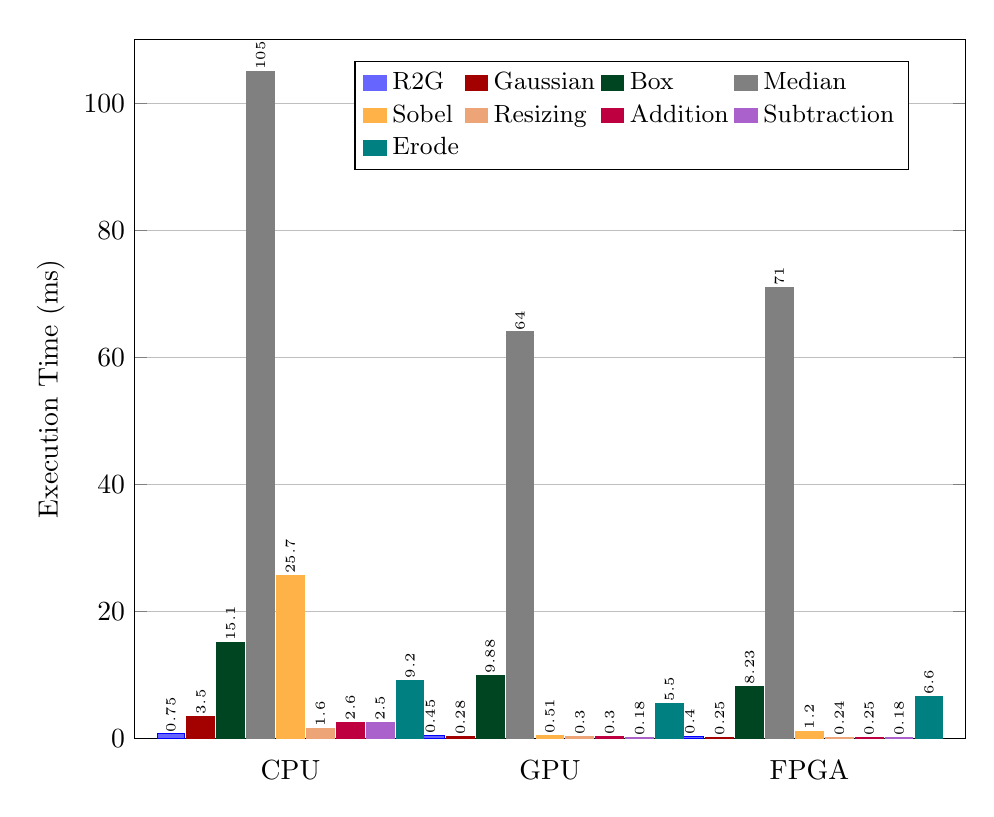
\begin{tikzpicture}
    \begin{axis}[
        width  = \linewidth,
        major x tick style = transparent,
        ybar=2*\pgflinewidth,
        ymin=0,ymax=100,
        bar width=10pt,
        enlarge y limits={upper=0.15},
        legend image code/.code={\draw[#1, draw=none] (0cm,-0.1cm) rectangle (0.3cm,0.1cm);
                },
        ymajorgrids = true,
        ylabel = {Execution Time (ms)},
        symbolic x coords={CPU,GPU,FPGA},
        xtick = data,
        nodes near coords,
        nodes near coords style={font=\tiny, anchor=west,rotate=90,inner xsep=0.5pt,black},
        scaled y ticks = false,
        enlarge x limits=0.30,
        legend cell align=left,
           enlarge y limits={upper=0.15},
    legend style={at={(0.2645,0.8915)},
                   anchor=west,legend columns=4, font=\small},
    ]
        \addplot[style={blue,fill=blue!60}]
            coordinates {(CPU, 0.75) (GPU,0.45) (FPGA,0.40)}; % RGB2GRAY
        \addplot[style={darkcandyapplered,fill=darkcandyapplered}]
             coordinates {(CPU,3.5) (GPU,0.28) (FPGA,0.25)}; % Gaussian
        \addplot[style={forestgreen,fill=forestgreen}]
             coordinates {(CPU,15.1) (GPU,9.88) (FPGA,8.23)}; % Box
        \addplot[style={gray,fill=gray}]
             coordinates {(CPU,105) (GPU,64) (FPGA,71)}; % Median
        \addplot[style={pastelorange,fill=pastelorange}]
             coordinates {(CPU,25.7) (GPU,0.51) (FPGA,1.2)}; % Sobel
        \addplot[style={oorange,fill=oorange}]
             coordinates {(CPU,1.6) (GPU,0.3) (FPGA,0.24)}; % resize
        \addplot[style={purple,fill=purple}]
             coordinates {(CPU,2.6) (GPU,0.30) (FPGA,0.25)}; % image add
        \addplot[style={richlavender,fill=richlavender}]
             coordinates {(CPU,2.5) (GPU,0.18) (FPGA,0.18)}; % image subtract
        \addplot[style={teal,fill=teal}]
             coordinates {(CPU,9.2) (GPU,5.5) (FPGA,6.6)}; % erode
        % \addplot[style={ppink,fill=ppink}]
        %      coordinates {(CPU,9.3) (GPU,5.7) (FPGA,6.8)}; % dilate
        % \addplot[style={bbrown,fill=bbrown}]
        %      coordinates {(CPU,43) (GPU,7) (FPGA,14)};  % Gamma           
        % \addplot[style={cyan,fill=cyan}]
        %      coordinates {(CPU,10.8) (GPU,0.25) (FPGA,0.20)}; % Placeholder for Linearization
        % \addplot[style={magenta,fill=magenta}]
        %      coordinates {(CPU,21.6) (GPU,0.19) (FPGA,0.28)}; % Placeholder for White Balance
        % \addplot[style={peridot,fill=peridot}]
        %      coordinates {(CPU,32) (GPU,0.44) (FPGA,1.1)}; % GEMM
        % \addplot[style={wenge,fill=wenge}]
        %      coordinates {(CPU,44) (GPU,24) (FPGA,18)}; % FFT
        % \addplot[style={yellow-green,fill=yellow-green}]
        %      coordinates {(CPU,1.8) (GPU,1.1) (FPGA,1.4)}; % STREAM
        % \addplot[style={brown,fill=brown}]
        %      coordinates {(CPU,3.3) (GPU,0.87) (FPGA,1.24)}; %Demosaicing
        \legend{R2G,Gaussian,Box, Median, Sobel,Resizing, Addition, Subtraction, Erode}
    \end{axis}
\end{tikzpicture}

%, Dilate, Gamma Corr., Linearization,White Balance,GEMM, FFT, STREAM, Demosaicing}    %\caption{Execution times for individual and combined algorithms.}
    \caption[SIFT Power Consumption]{Kernel (Lighter Colour) and Total Runtime (Solid Colour) Comparison of Individual Algorithms and Pipelines on each Hardware Platform. CPU(5900X) GPU(A2000) FPGA(Alveo U50).}
    \label{fig:IndividualRuntime}
\end{figure}

Regarding individual algorithm kernel runtimes, the results reveal that CPUs suffer poorly on high-complexity algorithms requiring more parallelisation. However, algorithms such as \texttt{RGB2Gray} and \texttt{Resize} exhibit better performance on the CPU than the GPU. The lower GPU runtime can be attributed to communication latency when allocating cores takes longer than the processing. The FPGA is shown to perform $1.81\times$ faster than the GPU and $1.79\times$ faster than the CPU in terms of kernel time for \texttt{RGB2GRAY}, \texttt{ Histogram Equalisation} and \texttt{Resize}) algorithms. However, the FPGA is less efficient for the \texttt{Gaussian} Filter algorithm, performing $1.2\times$ slower than the GPU. This inefficiency arises due to the limited number of logic blocks available on the FPGA, which are insufficient to fully parallelise the processing of all pixels. As a result, the FPGA cannot leverage its parallel processing capabilities to the same extent as the GPU, leading to longer kernel runtimes. This highlights a critical trade-off point where the FPGA's hardware constraints limit its performance on more demanding algorithms. In the case of deep learning algorithms, the GPU is $4.21\times$ \& $1.41\times$ faster than the CPU and FPGA, respectively. The convolutional layer, which contains the highest intensity of the operations in a CNN, benefits from the many-core GPU architecture. 

Slow GPU performance is observed for low-complexity algorithms where parallelisation cannot be effectively exploited. On the other hand, the bitstream pre-initialised U50 FPGA waits for incoming data, resulting in minimal latency, which can benefit image sensors streaming pixel data. In addition, the model initialisation takes, on average, $150ms$ on both CPU and GPU. Moreover, the U50 employs high-bandwidth memory, which can further improve memory-bound algorithms instead of the GDDR6 of the A2000 GPU. The runtime disparity between the \texttt{Total} and \texttt{Kernel} runtimes is due to the setup and initialisation times, including model/weight loading, computation graphs generation, memory allocation and data preprocessing. Therefore, GPU performs poorly, taking device and model initialisation into account, but this will only occur once.



According to Fig. \ref{fig:FPSEnergy}, the Frames Per Second (FPS) results show the impact of CNN algorithms. Large CNN architectures (e.g., Resnet-50 and InceptionV3) with deeper layers will involve many more operations, and additional processing modules and residual connections will also affect overall performance. In relation to energy consumption, the FPGA consumed the least amount of energy per operation for all algorithms. On average, the FPGA is $7.63\times$ and $2.60\times$ more energy efficient than the CPU and GPU. Although the GPU has a higher thermal design power (TDP) than the CPU, the time it takes to execute the algorithm is much lower, resulting in lower overall energy use despite the higher power draw. Algorithms that contain many operations, such as ML and Gaussian, show that the GPU consumes less energy than the CPU.

Referring to the profiling results, the partitioning approach will place the pre-processing algorithms on the FPGA to maximise energy efficiency. In contrast, the deep learning algorithm will be deployed on the GPU for runtime. This strategy takes advantage of the FPGA's low initialisation latency and memory coupled with the GPUs parallel processing capability.




\begin{figure}[tb]
    \centering
    \begin{tabular}{cc}
    \resizebox{0.5\columnwidth}{!}{\pgfplotsset{width=0.6\linewidth,compat=1.3}
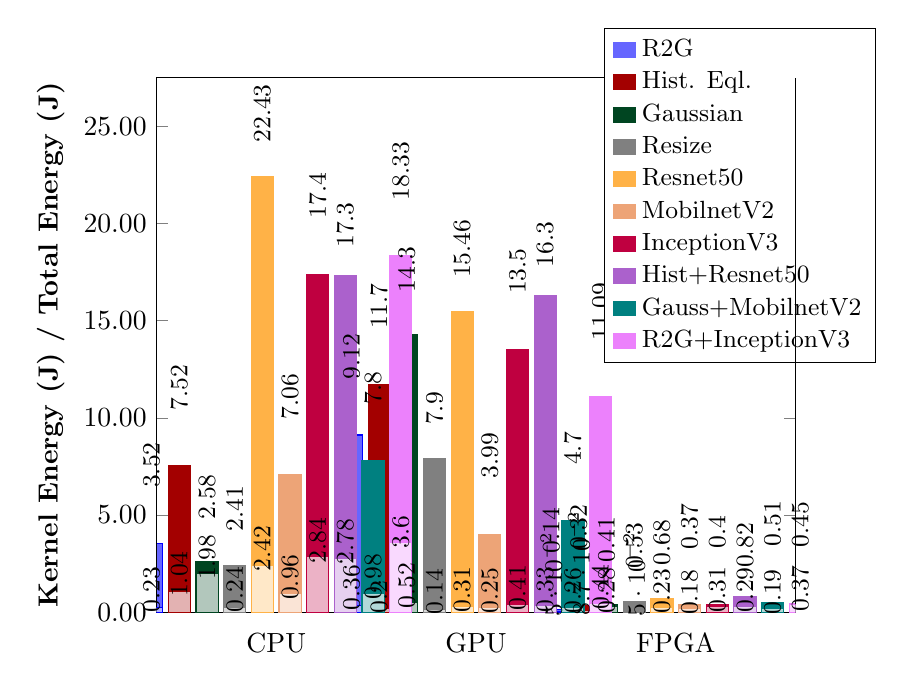
\begin{tikzpicture}
    % Kernel Energy Axis
    \begin{axis}[
        width  = 0.8\linewidth,
        major x tick style = transparent,
        ybar,
        ymin=0, ymax=25,
        bar width=8pt,
        enlarge y limits={upper=0.15},
        legend image code/.code={\draw[#1, draw=none] (0cm,-0.1cm) rectangle (0.3cm,0.1cm);},
        ymajorgrids = false,
        ylabel = {\textbf{Kernel Energy (J) / Total Energy (J)}},
        symbolic x coords={CPU,GPU,FPGA},
        xtick = data,
        nodes near coords,
        nodes near coords style={font=\small, anchor=west,rotate=90,inner xsep=0.9pt,black},
        yticklabel style={/pgf/number format/fixed,/pgf/number format/precision=2,/pgf/number format/fixed zerofill}, % Ensure full numbers are shown
        scaled y ticks = false,
        enlarge x limits=0.30,
        legend cell align=left,
        legend style={at={(0.7,0.78)},
                       anchor=west,legend columns=1, font=\small},
        axis on top,
    ]
        % Total Energy Data Plots
        \addplot[style={blue,fill=blue!60}, every node near coord/.append style={rotate=0, anchor=west,inner xsep=20pt}]
            coordinates {(CPU, 3.52) (GPU, 9.116) (FPGA, 0.14)}; % RGB2GRAY
        \addplot[style={darkcandyapplered,fill=darkcandyapplered}, every node near coord/.append style={rotate=0, anchor=west,inner xsep=20pt}]
            coordinates {(CPU, 7.52) (GPU, 11.7) (FPGA, 0.32)}; % Histogram Equalisation
        \addplot[style={forestgreen,fill=forestgreen}, every node near coord/.append style={rotate=0, anchor=west,inner xsep=15pt}]
            coordinates {(CPU, 2.58) (GPU, 14.3) (FPGA, 0.41)}; % Gaussian Filter (7x7)
        \addplot[style={gray,fill=gray}, every node near coord/.append style={rotate=0, anchor=west,inner xsep=12pt}]
            coordinates {(CPU, 2.41) (GPU, 7.90) (FPGA, 0.53)}; % Resize
        \addplot[style={pastelorange,fill=pastelorange}, every node near coord/.append style={rotate=0, anchor=west,inner xsep=12pt}]
            coordinates {(CPU, 22.43) (GPU, 15.46) (FPGA, 0.68)}; % Resnet50
        \addplot[style={oorange,fill=oorange}, every node near coord/.append style={rotate=0, anchor=west,inner xsep=20pt}]
            coordinates {(CPU, 7.06) (GPU, 3.99) (FPGA, 0.37)}; % MobilnetV2
        \addplot[style={purple,fill=purple}, every node near coord/.append style={rotate=0, anchor=west,inner xsep=20pt}]
            coordinates {(CPU, 17.4) (GPU, 13.50) (FPGA, 0.40)}; % InceptionV3
        \addplot[style={richlavender,fill=richlavender}, every node near coord/.append style={rotate=0, anchor=west,inner xsep=10pt}]
            coordinates {(CPU, 17.30) (GPU, 16.30) (FPGA, 0.82)}; % Histogram Equalisation + ResNet-50
        \addplot[style={teal,fill=teal}, every node near coord/.append style={rotate=0, anchor=west,inner xsep=20pt}]
            coordinates {(CPU, 7.80) (GPU, 4.70) (FPGA, 0.51)}; % Gaussian Filter + MobilnetV2
        
        \addplot[style={ppink,fill=ppink}, every node near coord/.append style={rotate=0, anchor=west,inner xsep=20pt}]
            coordinates {(CPU, 18.33) (GPU, 11.09) (FPGA, 0.45)}; % RGB2Gray + InceptionV3

        \legend{R2G, Hist. Eql., Gaussian, Resize, Resnet50, MobilnetV2, InceptionV3, Hist+Resnet50, Gauss+MobilnetV2, R2G+InceptionV3}
    \end{axis}

    % Kernel Energy Axis
    \begin{axis}[
        width  = 0.8\linewidth,
        major x tick style = transparent,
        ybar,
        ymin=0, ymax=25,
        bar width=8pt,
        enlarge y limits={upper=0.15},
        legend image code/.code={\draw[#1, draw=none] (0cm,-0.1cm) rectangle (0.3cm,0.1cm);},
        ymajorgrids = false,
        ylabel = {\textbf{}},
        axis y line*=right,
        axis x line=none,
        symbolic x coords={CPU,GPU,FPGA},
        xtick = \empty,
        ytick style = {draw=none}, % Hides the y-axis ticks
        yticklabels = {}, % Hides the y-axis labels
        nodes near coords,
        nodes near coords style={font=\small, anchor=west,rotate=90,inner xsep=0.5pt,black,shift={(-2.5pt,0pt)}}, % Adjust shift as needed
        yticklabel style={/pgf/number format/fixed,/pgf/number format/precision=2,/pgf/number format/fixed zerofill}, % Ensure full numbers are shown
        scaled y ticks = false,
        enlarge x limits=0.30,
        legend cell align=left,
        legend style={at={(0.5,1.05)},
                       anchor=west,legend columns=4, font=\small},
    ]
    
        % Kernel Energy Data Plots
        \addplot[style={blue,fill=blue!30},]
            coordinates {(CPU, 0.23) (GPU, 0.36) (FPGA, 0.05)}; % RGB2GRAY
        \addplot[style={darkcandyapplered,fill=darkcandyapplered!30}]
            coordinates {(CPU, 1.04) (GPU, 0.20) (FPGA, 0.087)}; % Histogram Equalisation
        \addplot[style={forestgreen,fill=forestgreen!30}, every node near coord/.append style={rotate=0, anchor=west,inner xsep=0pt}]
            coordinates {(CPU, 1.98) (GPU, 0.52) (FPGA, 0.28)}; % Gaussian Filter (7x7)
        \addplot[style={gray,fill=gray!30}]
            coordinates {(CPU, 0.24) (GPU, 0.14) (FPGA, 0.05)}; % Resize
        \addplot[style={pastelorange,fill=pastelorange!30},every node near coord/.append style={rotate=0, anchor=west,inner xsep=0pt}]
            coordinates {(CPU, 2.42) (GPU, 0.31) (FPGA, 0.23)}; % Resnet50
        \addplot[style={oorange,fill=oorange!30},every node near coord/.append style={rotate=0, anchor=west,inner xsep=0pt}]
            coordinates {(CPU, 0.96) (GPU, 0.25) (FPGA, 0.18)}; % MobilnetV2
        \addplot[style={purple,fill=purple!30},every node near coord/.append style={rotate=0, anchor=west,inner xsep=0pt}]
            coordinates {(CPU, 2.84) (GPU, 0.41) (FPGA, 0.31)}; % InceptionV3
        \addplot[style={richlavender,fill=richlavender!30},every node near coord/.append style={rotate=0, anchor=west,inner xsep=0pt}]
            coordinates {(CPU, 2.78) (GPU, 0.33) (FPGA, 0.29)}; % Histogram Equalisation + ResNet-50
        \addplot[style={teal,fill=teal!30},every node near coord/.append style={rotate=0, anchor=west,inner xsep=0pt}]
            coordinates {(CPU, 0.98) (GPU, 0.26) (FPGA, 0.19)}; % Gaussian Filter + MobilnetV2
        \addplot[style={ppink,fill=ppink!30},every node near coord/.append style={rotate=0, anchor=west,inner xsep=0pt}]
            coordinates {(CPU, 3.60) (GPU, 0.44) (FPGA, 0.37)}; % RGB2Gray + InceptionV3

        % \legend{R2G Total, Gaussian Total, Box Total, Median Total, Sobel Total, Resize Total, Addition Total, Subtraction Total, Erode Total, Dilate Total, Gamma Total}
        
    \end{axis}
\end{tikzpicture}
} &
    \resizebox{0.5\columnwidth}{!}{\pgfplotsset{width=0.6\linewidth,compat=1.3}
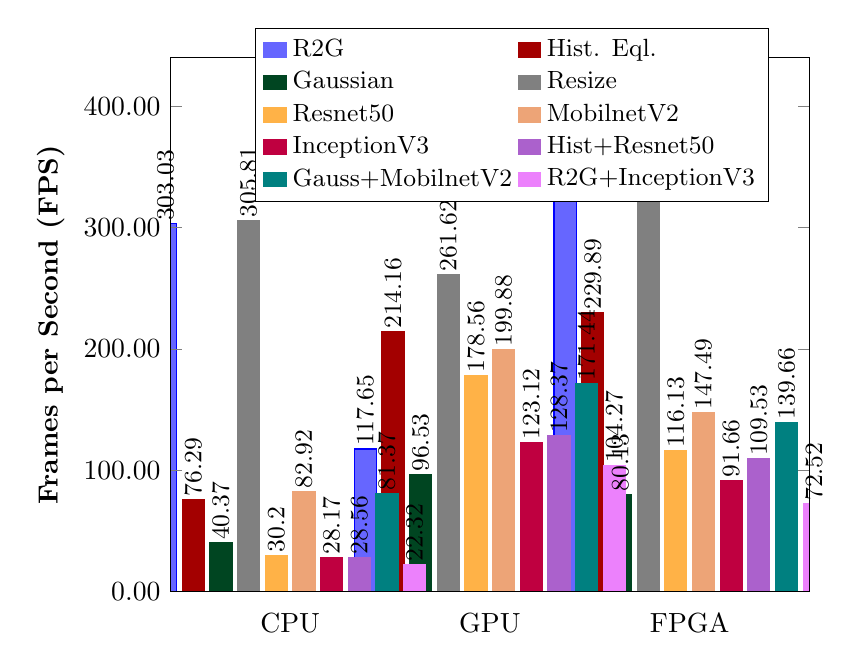
\begin{tikzpicture}
    % FPS Axis
    \begin{axis}[
        width  = 0.8\linewidth,
        major x tick style = transparent,
        ybar,
        ymin=0, ymax=400,
        bar width=8pt,
        enlarge y limits={upper=0.15},
        legend image code/.code={\draw[#1, draw=none] (0cm,-0.1cm) rectangle (0.3cm,0.1cm);},
        ymajorgrids = false,
        ylabel = {\textbf{Frames per Second (FPS)}},
        symbolic x coords={CPU,GPU,FPGA},
        xtick = data,
        nodes near coords,
        nodes near coords style={font=\small, anchor=west,rotate=90,inner xsep=0.9pt,black},
        yticklabel style={/pgf/number format/fixed,/pgf/number format/precision=2,/pgf/number format/fixed zerofill}, % Ensure full numbers are shown
        scaled y ticks = false,
        enlarge x limits=0.30,
        legend cell align=left,
        legend style={at={(0.132,0.893)},
                       anchor=west,legend columns=2, font=\small},
        axis on top,
    ]
        % FPS Data Plots
        \addplot[style={blue,fill=blue!60}, every node near coord/.append style={rotate=0, anchor=west,inner xsep=0.9pt}]
            coordinates {(CPU, 303.03) (GPU, 117.65) (FPGA, 344.83)}; % RGB2GRAY
        \addplot[style={darkcandyapplered,fill=darkcandyapplered}, every node near coord/.append style={rotate=0, anchor=west,inner xsep=0.9pt}]
            coordinates {(CPU, 76.29) (GPU, 214.16) (FPGA, 229.89)}; % Histogram Equalisation
        \addplot[style={forestgreen,fill=forestgreen}, every node near coord/.append style={rotate=0, anchor=west,inner xsep=0.9pt}]
            coordinates {(CPU, 40.37) (GPU, 96.53) (FPGA, 80.13)}; % Gaussian Filter (7x7)
        \addplot[style={gray,fill=gray}, every node near coord/.append style={rotate=0, anchor=west,inner xsep=0.9pt}]
            coordinates {(CPU, 305.81) (GPU, 261.62) (FPGA, 378.79)}; % Resize
        \addplot[style={pastelorange,fill=pastelorange}, every node near coord/.append style={rotate=0, anchor=west,inner xsep=0.9pt}]
            coordinates {(CPU, 30.20) (GPU, 178.56) (FPGA, 116.13)}; % Resnet50
        \addplot[style={oorange,fill=oorange}, every node near coord/.append style={rotate=0, anchor=west,inner xsep=0.9pt}]
            coordinates {(CPU, 82.92) (GPU, 199.88) (FPGA, 147.49)}; % MobilnetV2
        \addplot[style={purple,fill=purple}, every node near coord/.append style={rotate=0, anchor=west,inner xsep=0.9pt}]
            coordinates {(CPU, 28.17) (GPU, 123.12) (FPGA, 91.66)}; % InceptionV3
        \addplot[style={richlavender,fill=richlavender}, every node near coord/.append style={rotate=0, anchor=west,inner xsep=0.9pt}]
            coordinates {(CPU, 28.56) (GPU, 128.37) (FPGA, 109.53)}; % Histogram Equalisation + ResNet-50
        \addplot[style={teal,fill=teal}, every node near coord/.append style={rotate=0, anchor=west,inner xsep=0.9pt}]
            coordinates {(CPU, 81.37) (GPU, 171.44) (FPGA, 139.66)}; % Gaussian Filter + MobilnetV2
        \addplot[style={ppink,fill=ppink}, every node near coord/.append style={rotate=0, anchor=west,inner xsep=0.9pt}]
            coordinates {(CPU, 22.32) (GPU, 104.27) (FPGA, 72.52)}; % RGB2Gray + InceptionV3

        \legend{R2G, Hist. Eql., Gaussian, Resize, Resnet50, MobilnetV2, InceptionV3, Hist+Resnet50, Gauss+MobilnetV2, R2G+InceptionV3}
    \end{axis}
\end{tikzpicture}
} \\    a & b 
    \end{tabular}
    \caption{Algorithmic a) Energy Consumption Comparison of Individual Algorithms, Pipelines and b) Frames per Second on each Hardware Platform. CPU(5900x) GPU(A2000) FPGA(Alveo U50).}
    \label{fig:FPSEnergy}
\end{figure}



% \begin{figure}
%     \centering
% \resizebox{0.7\linewidth}{!}{\pgfplotsset{width=0.6\linewidth,compat=1.3}
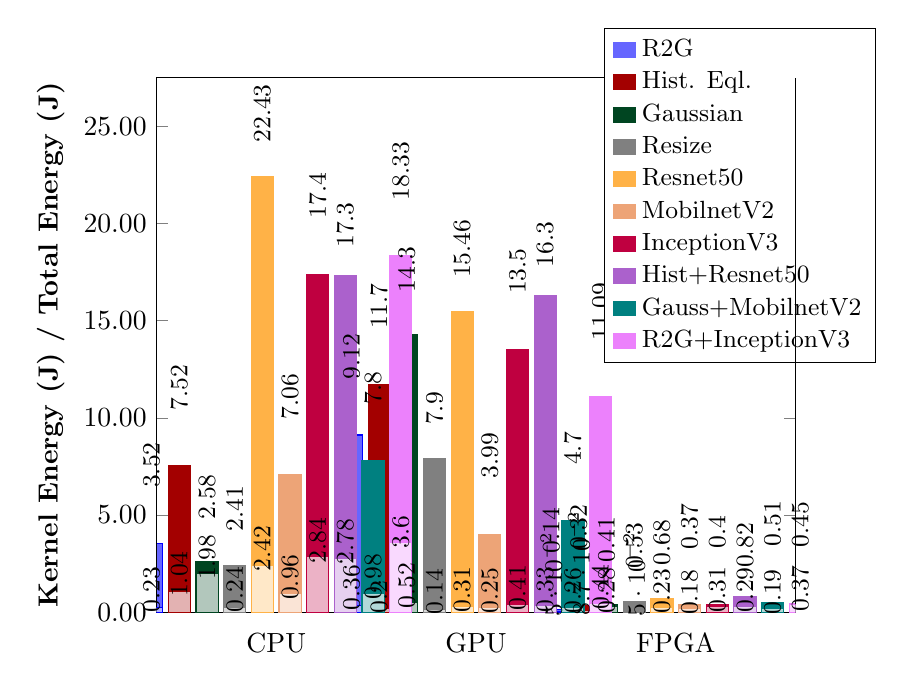
\begin{tikzpicture}
    % Kernel Energy Axis
    \begin{axis}[
        width  = 0.8\linewidth,
        major x tick style = transparent,
        ybar,
        ymin=0, ymax=25,
        bar width=8pt,
        enlarge y limits={upper=0.15},
        legend image code/.code={\draw[#1, draw=none] (0cm,-0.1cm) rectangle (0.3cm,0.1cm);},
        ymajorgrids = false,
        ylabel = {\textbf{Kernel Energy (J) / Total Energy (J)}},
        symbolic x coords={CPU,GPU,FPGA},
        xtick = data,
        nodes near coords,
        nodes near coords style={font=\small, anchor=west,rotate=90,inner xsep=0.9pt,black},
        yticklabel style={/pgf/number format/fixed,/pgf/number format/precision=2,/pgf/number format/fixed zerofill}, % Ensure full numbers are shown
        scaled y ticks = false,
        enlarge x limits=0.30,
        legend cell align=left,
        legend style={at={(0.7,0.78)},
                       anchor=west,legend columns=1, font=\small},
        axis on top,
    ]
        % Total Energy Data Plots
        \addplot[style={blue,fill=blue!60}, every node near coord/.append style={rotate=0, anchor=west,inner xsep=20pt}]
            coordinates {(CPU, 3.52) (GPU, 9.116) (FPGA, 0.14)}; % RGB2GRAY
        \addplot[style={darkcandyapplered,fill=darkcandyapplered}, every node near coord/.append style={rotate=0, anchor=west,inner xsep=20pt}]
            coordinates {(CPU, 7.52) (GPU, 11.7) (FPGA, 0.32)}; % Histogram Equalisation
        \addplot[style={forestgreen,fill=forestgreen}, every node near coord/.append style={rotate=0, anchor=west,inner xsep=15pt}]
            coordinates {(CPU, 2.58) (GPU, 14.3) (FPGA, 0.41)}; % Gaussian Filter (7x7)
        \addplot[style={gray,fill=gray}, every node near coord/.append style={rotate=0, anchor=west,inner xsep=12pt}]
            coordinates {(CPU, 2.41) (GPU, 7.90) (FPGA, 0.53)}; % Resize
        \addplot[style={pastelorange,fill=pastelorange}, every node near coord/.append style={rotate=0, anchor=west,inner xsep=12pt}]
            coordinates {(CPU, 22.43) (GPU, 15.46) (FPGA, 0.68)}; % Resnet50
        \addplot[style={oorange,fill=oorange}, every node near coord/.append style={rotate=0, anchor=west,inner xsep=20pt}]
            coordinates {(CPU, 7.06) (GPU, 3.99) (FPGA, 0.37)}; % MobilnetV2
        \addplot[style={purple,fill=purple}, every node near coord/.append style={rotate=0, anchor=west,inner xsep=20pt}]
            coordinates {(CPU, 17.4) (GPU, 13.50) (FPGA, 0.40)}; % InceptionV3
        \addplot[style={richlavender,fill=richlavender}, every node near coord/.append style={rotate=0, anchor=west,inner xsep=10pt}]
            coordinates {(CPU, 17.30) (GPU, 16.30) (FPGA, 0.82)}; % Histogram Equalisation + ResNet-50
        \addplot[style={teal,fill=teal}, every node near coord/.append style={rotate=0, anchor=west,inner xsep=20pt}]
            coordinates {(CPU, 7.80) (GPU, 4.70) (FPGA, 0.51)}; % Gaussian Filter + MobilnetV2
        
        \addplot[style={ppink,fill=ppink}, every node near coord/.append style={rotate=0, anchor=west,inner xsep=20pt}]
            coordinates {(CPU, 18.33) (GPU, 11.09) (FPGA, 0.45)}; % RGB2Gray + InceptionV3

        \legend{R2G, Hist. Eql., Gaussian, Resize, Resnet50, MobilnetV2, InceptionV3, Hist+Resnet50, Gauss+MobilnetV2, R2G+InceptionV3}
    \end{axis}

    % Kernel Energy Axis
    \begin{axis}[
        width  = 0.8\linewidth,
        major x tick style = transparent,
        ybar,
        ymin=0, ymax=25,
        bar width=8pt,
        enlarge y limits={upper=0.15},
        legend image code/.code={\draw[#1, draw=none] (0cm,-0.1cm) rectangle (0.3cm,0.1cm);},
        ymajorgrids = false,
        ylabel = {\textbf{}},
        axis y line*=right,
        axis x line=none,
        symbolic x coords={CPU,GPU,FPGA},
        xtick = \empty,
        ytick style = {draw=none}, % Hides the y-axis ticks
        yticklabels = {}, % Hides the y-axis labels
        nodes near coords,
        nodes near coords style={font=\small, anchor=west,rotate=90,inner xsep=0.5pt,black,shift={(-2.5pt,0pt)}}, % Adjust shift as needed
        yticklabel style={/pgf/number format/fixed,/pgf/number format/precision=2,/pgf/number format/fixed zerofill}, % Ensure full numbers are shown
        scaled y ticks = false,
        enlarge x limits=0.30,
        legend cell align=left,
        legend style={at={(0.5,1.05)},
                       anchor=west,legend columns=4, font=\small},
    ]
    
        % Kernel Energy Data Plots
        \addplot[style={blue,fill=blue!30},]
            coordinates {(CPU, 0.23) (GPU, 0.36) (FPGA, 0.05)}; % RGB2GRAY
        \addplot[style={darkcandyapplered,fill=darkcandyapplered!30}]
            coordinates {(CPU, 1.04) (GPU, 0.20) (FPGA, 0.087)}; % Histogram Equalisation
        \addplot[style={forestgreen,fill=forestgreen!30}, every node near coord/.append style={rotate=0, anchor=west,inner xsep=0pt}]
            coordinates {(CPU, 1.98) (GPU, 0.52) (FPGA, 0.28)}; % Gaussian Filter (7x7)
        \addplot[style={gray,fill=gray!30}]
            coordinates {(CPU, 0.24) (GPU, 0.14) (FPGA, 0.05)}; % Resize
        \addplot[style={pastelorange,fill=pastelorange!30},every node near coord/.append style={rotate=0, anchor=west,inner xsep=0pt}]
            coordinates {(CPU, 2.42) (GPU, 0.31) (FPGA, 0.23)}; % Resnet50
        \addplot[style={oorange,fill=oorange!30},every node near coord/.append style={rotate=0, anchor=west,inner xsep=0pt}]
            coordinates {(CPU, 0.96) (GPU, 0.25) (FPGA, 0.18)}; % MobilnetV2
        \addplot[style={purple,fill=purple!30},every node near coord/.append style={rotate=0, anchor=west,inner xsep=0pt}]
            coordinates {(CPU, 2.84) (GPU, 0.41) (FPGA, 0.31)}; % InceptionV3
        \addplot[style={richlavender,fill=richlavender!30},every node near coord/.append style={rotate=0, anchor=west,inner xsep=0pt}]
            coordinates {(CPU, 2.78) (GPU, 0.33) (FPGA, 0.29)}; % Histogram Equalisation + ResNet-50
        \addplot[style={teal,fill=teal!30},every node near coord/.append style={rotate=0, anchor=west,inner xsep=0pt}]
            coordinates {(CPU, 0.98) (GPU, 0.26) (FPGA, 0.19)}; % Gaussian Filter + MobilnetV2
        \addplot[style={ppink,fill=ppink!30},every node near coord/.append style={rotate=0, anchor=west,inner xsep=0pt}]
            coordinates {(CPU, 3.60) (GPU, 0.44) (FPGA, 0.37)}; % RGB2Gray + InceptionV3

        % \legend{R2G Total, Gaussian Total, Box Total, Median Total, Sobel Total, Resize Total, Addition Total, Subtraction Total, Erode Total, Dilate Total, Gamma Total}
        
    \end{axis}
\end{tikzpicture}
}    %\caption{Execution times for individual and combined algorithms.}
%     \caption[SIFT Power Consumption]{Energy Consumption Comparison of Individual Algorithms and Pipelines on each Hardware Platform.}
%     \label{fig:IndividualPower}
% \end{figure}




\section{Experimental Setup}
\begin{minipage}{0.4\linewidth}
\begin{figure}[H]
    \centering
    \includegraphics[width=\linewidth]{images/hardware.png} % Adjust the image width to fit the minipage
    \caption{Heterogeneous System Enviroment}
    \label{fig:HeterogenousHardware}
\end{figure}
\end{minipage}%
\hspace{5mm}
\begin{minipage}{0.6\linewidth}
\begin{table}[H]
\centering
\setlength{\extrarowheight}{0pt}
\addtolength{\extrarowheight}{\aboverulesep}
\addtolength{\extrarowheight}{\belowrulesep}
\setlength{\aboverulesep}{0pt}
\setlength{\belowrulesep}{0pt}
\caption{Hardware/Software Environment}
\label{tab:HWEnvironment}
\resizebox{\linewidth}{!}{%
\begin{tabular}{c|c|c|c} 
\toprule
\rowcolor[rgb]{0.753,0.753,0.753} \textbf{Accelerator} & \textbf{Hardware} & \begin{tabular}[c]{@{}>{\cellcolor[rgb]{0.753,0.753,0.753}}c@{}}\textbf{Language /}\\\textbf{Library}\end{tabular} & \multicolumn{1}{c|}{\begin{tabular}[c]{@{}>{\cellcolor[rgb]{0.753,0.753,0.753}}c@{}}\textbf{Energy}\\\textbf{Measurement}\end{tabular}} \\ 
\cmidrule{1-3}\cline{4-4}
CPU & \begin{tabular}[c]{@{}c@{}}AMD 5900x \\ (4.8 GHz)\end{tabular} & \begin{tabular}[c]{@{}c@{}}Python / \\Pytorch 2.4\end{tabular} & RAPL \\ 
\cmidrule{1-3}\cline{4-4}
GPU & \begin{tabular}[c]{@{}c@{}}Nvidia A2000 \\ (1200 MHz)\end{tabular} & \begin{tabular}[c]{@{}c@{}}Python / \\Pytorch 2.4\end{tabular} & Nvidia SMI \\ 
\cmidrule{1-3}\cline{4-4}
FPGA & \begin{tabular}[c]{@{}c@{}}U50 \\ (300 MHz)\end{tabular} & \begin{tabular}[c]{@{}c@{}}HLS (C++) / \\Vitis Vision\end{tabular} & Xbutil \\
\bottomrule
\end{tabular}
}
\end{table}
\end{minipage}
\newline 
The proposed partitioning is evaluated using a heterogeneous platform containing various hardware components and their software, as shown in Table \ref{tab:HWEnvironment} and Fig. \ref{fig:HeterogenousHardware}. The heterogeneous platform, integrates a CPU, GPU and FPGA that are connected with a PCIe Gen3 interface. The operating system used for the experiment is Linux Ubuntu with loaded DMA drivers provided by the manufacturer.

\textbf{Dataset.} The test images used in the experiments are from LIU4K-v2 dataset \cite{LiuliuYan19}, which is a high resolution data-set that includes 2000 $3840\times2160$ images. The images contain a variety of backgrounds and objects. 


\subsection{Measurement Metrics}
\subsubsection{Execution time}
The evaluation of overall system performance considers both latency and compute factors, reporting performance metrics for total time, inference, and other significant layers while using floating-point 16-bit precision. The runtime is measured using the host platform's built-in time libraries. The algorithm runtime is collected from executing $1000\times$ and averaged.  

The U50 FPGA, time measurements are captured using the Xilinx Vitis analyser built-in performance counters. On the GPU, CUDA events are utilised to measure time. CUDA events work by recording timestamps at specific points in the code. These timestamps are captured by calling \verb|cudaEventRecord()| at the code's desired start and stop points. The \verb|cudaEventElapsedTime()| function is then used to calculate the elapsed time between these two events. CUDA events provide high-resolution timing by using the GPU's internal clock, allowing for precise measurement of kernel execution times and other GPU operations with minimal overhead. For the CPU, a C++ library is employed to measure execution time. This library offers high-resolution timing functions such as \verb|std::chrono::high_resolution_clock| to capture start and end times, providing precise timing information for the CPU operations. The frame per second (FPS) metric is computed using Eq. \ref{eq:FPS}: 

\begin{equation}\label{eq:FPS}
\text{FPS}= 1/\text{Execution Time}.
\end{equation}

\subsubsection{Power Consumption}

Taking a device's instantaneous power or TDP is inaccurate since power consumption varies depending on the workload. Therefore, measuring power over the time it takes for the algorithm to execute improves accuracy as opposed to using just fixed Wattage. A script is developed to start and stop the measurements during the algorithm's execution. The mean wattage is averaged and multiplied by the time to determine the energy consumed in Joules (J). The energy consumption is obtained using Eq. (\ref{eq:Energy}), where \textit{E} is energy, \textit{P} represents power, and \textit{t} time.

\begin{equation}\label{eq:Energy}
E = P \times t
\end{equation}

Power measurements are taken using software-based platform-specific tools. For the CPU, \texttt{RAPL} collects energy consumption using a script that reads the initial and final energy values. For the GPU, \texttt{nvidia-smi} obtains power readings at the same interval. For the U50 FPGA, \texttt{xbutil} monitors power consumption. The power readings are then averaged to provide an accurate measure of energy consumption during the algorithm's execution.

\subsubsection{Accuracy}
The accuracy of the proposed system for CNN classification is evaluated using a straightforward metric: the ratio of correctly classified images to the total number of images in the test dataset. This metric provides a clear measure of how well the CNN model performs in terms of correctly identifying the class labels of the input images. The accuracy is calculated using Eq. \ref{eq
}:

\begin{equation}\label{eq
}
\text{Accuracy} = \frac{\text{Number of Correct Predictions}}{\text{Total Number of Predictions}}
\end{equation}

% RMSE is used to compare the accuracy of the output images from each algorithm, across hardware platforms. RMSE quantifies the differences between predicted and actual pixel values in image processing tasks. It is calculated using Eq. \ref{RSME}:

% \begin{equation}\label{RSME}
% \text{RMSE} = \sqrt{\frac{1}{N} \sum_{i=1}^{N} (I_{pred}(i) - I_{actual}(i))^2}
% \end{equation}

% where \( N \) is the total number of pixels, \( I_{\text{pred}}(i) \) is the predicted pixel value, and \( I_{\text{actual}}(i) \) is the actual pixel value.



\section{Results}
\begin{figure}[tb]
    \centering
    \begin{tabular}{cc}
    \resizebox{0.48\columnwidth}{!}{\pgfplotsset{width=0.6\linewidth,compat=1.3}
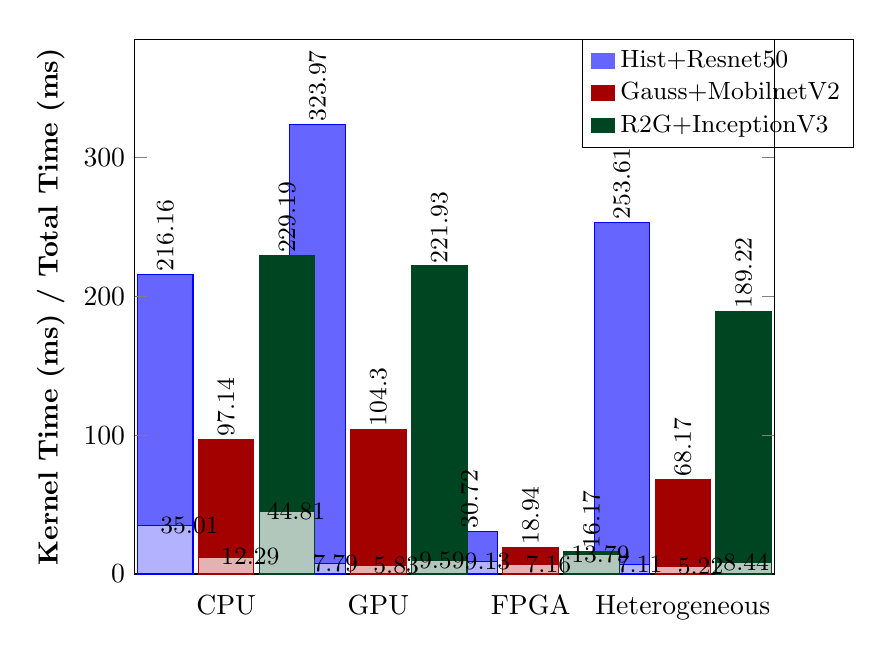
\begin{tikzpicture}
    % Kernel Time Axis
    \begin{axis}[
        width  = 0.8\linewidth,
        major x tick style = transparent,
        ybar,
        ymin=0, ymax=350,
        bar width=20pt,
        enlarge y limits={upper=0.15},
        legend image code/.code={\draw[#1, draw=none] (0cm,-0.1cm) rectangle (0.3cm,0.1cm);},
        ymajorgrids = false,
        ylabel = {\textbf{Kernel Time (ms) / Total Time (ms)}},
        symbolic x coords={CPU,GPU,FPGA,Heterogeneous},
        xtick = data,
        nodes near coords,
        nodes near coords style={font=\small, anchor=west,rotate=90,inner xsep=0.9pt,black},
        scaled y ticks = false,
        enlarge x limits=0.20,
        legend cell align=left,
        legend style={at={(0.7,0.9)},
                       anchor=west,legend columns=1, font=\small},
        axis on top,
    ]
        % Total Time Data Plots
        \addplot[style={blue,fill=blue!60}, every node near coord/.append style={rotate=0, anchor=west,inner xsep=0.9pt}]
            coordinates {(CPU, 216.16) (GPU, 323.97) (FPGA, 30.72) (Heterogeneous, 253.61)}; % Histogram Equalisation + ResNet-50
        \addplot[style={darkcandyapplered,fill=darkcandyapplered}, every node near coord/.append style={rotate=0, anchor=west,inner xsep=0.9pt}]
            coordinates {(CPU, 97.14) (GPU, 104.30) (FPGA, 18.94) (Heterogeneous, 68.17)}; % Gaussian Filter + MobilnetV2
        \addplot[style={forestgreen,fill=forestgreen}, every node near coord/.append style={rotate=0, anchor=west,inner xsep=0.9pt}]
            coordinates {(CPU, 229.19) (GPU, 221.93) (FPGA, 16.17) (Heterogeneous, 189.22)}; % RGB2Gray + InceptionV3
        \legend{Hist+Resnet50, Gauss+MobilnetV2, R2G+InceptionV3}
    \end{axis}

    % Total Time Axis
    \begin{axis}[
        width  = 0.8\linewidth,
        major x tick style = transparent,
        ybar,
        ymin=0, ymax=350,
        bar width=20pt,
        enlarge y limits={upper=0.15},
        legend image code/.code={\draw[#1, draw=none] (0cm,-0.1cm) rectangle (0.3cm,0.1cm);},
        ymajorgrids = false,
        ylabel = {\textbf{}},
        axis y line*=right,
        axis x line=none,
        symbolic x coords={CPU,GPU,FPGA,Heterogeneous},
        xtick = \empty,
        ytick style = {draw=none}, % Hides the y-axis ticks
        yticklabels = {}, % Hides the y-axis labels
        nodes near coords,
        nodes near coords style={font=\small, anchor=west,rotate=0,inner xsep=0.5pt,black,shift={(-2.5pt,0pt)}}, % Adjust shift as needed
        scaled y ticks = false,
        enlarge x limits=0.20,
        legend cell align=left,
        legend style={at={(0.5,1.05)},
                       anchor=west,legend columns=4, font=\small},
    ]
        % Kernel Time Data Plots
        \addplot[style={blue,fill=blue!30}]
            coordinates {(CPU, 35.01) (GPU, 7.79) (FPGA, 9.13) (Heterogeneous, 7.11)}; % Histogram Equalisation + ResNet-50
        \addplot[style={darkcandyapplered,fill=darkcandyapplered!30}]
            coordinates {(CPU, 12.29) (GPU, 5.83) (FPGA, 7.16) (Heterogeneous, 5.22)}; % Gaussian Filter + MobilnetV2
        \addplot[style={forestgreen,fill=forestgreen!30}, every node near coord/.append style={rotate=0, anchor=west,inner xsep=-5pt}]
            coordinates {(CPU, 44.81) (GPU, 9.59) (FPGA, 13.79) (Heterogeneous, 8.44)}; % RGB2Gray + InceptionV3
        % \legend{Hist+Resnet50, Gauss+MobilnetV2, R2G+InceptionV3}
    \end{axis}
\end{tikzpicture}
} &
    \resizebox{0.49\columnwidth}{!}{\pgfplotsset{width=0.6\linewidth,compat=1.3}
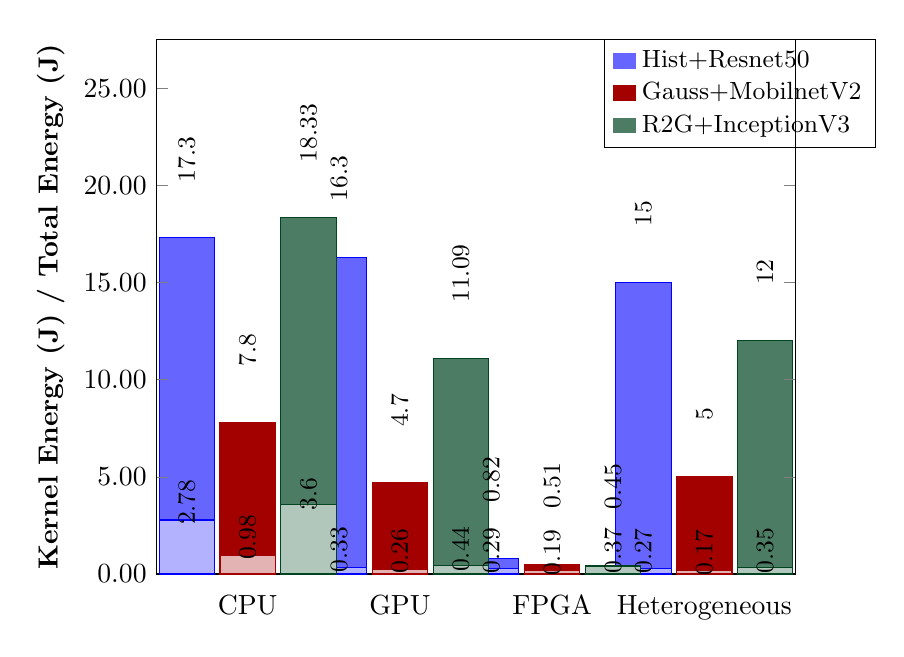
\begin{tikzpicture}
    % Kernel Energy Axis
    \begin{axis}[
        width  = 0.8\linewidth,
        major x tick style = transparent,
        ybar,
        ymin=0, ymax=25,
        bar width=20pt,
        enlarge y limits={upper=0.15},
        legend image code/.code={\draw[#1, draw=none] (0cm,-0.1cm) rectangle (0.3cm,0.1cm);},
        ymajorgrids = false,
        ylabel = {\textbf{Kernel Energy (J) / Total Energy (J)}},
        symbolic x coords={CPU,GPU,FPGA,Heterogeneous},
        xtick = data,
        nodes near coords,
        nodes near coords style={font=\small, anchor=west,rotate=90,inner xsep=0.9pt,black},
        yticklabel style={/pgf/number format/fixed,/pgf/number format/precision=2,/pgf/number format/fixed zerofill}, % Ensure full numbers are shown
        scaled y ticks = false,
        enlarge x limits=0.20,
        legend cell align=left,
        legend style={at={(0.7,0.9)},
                       anchor=west,legend columns=1, font=\small},
        axis on top,
    ]
        % Total Energy Data Plots
        \addplot[style={blue,fill=blue!60}, every node near coord/.append style={rotate=0, anchor=west,inner xsep=20pt}]
            coordinates {(CPU, 17.30) (GPU, 16.30) (FPGA, 0.82) (Heterogeneous, 15.00)}; % Histogram Equalisation + ResNet-50
        \addplot[style={darkcandyapplered,fill=darkcandyapplered}, every node near coord/.append style={rotate=0, anchor=west,inner xsep=20pt}]
            coordinates {(CPU, 7.80) (GPU, 4.70) (FPGA, 0.51) (Heterogeneous, 5.00)}; % Gaussian Filter + MobilnetV2
        \addplot[style={forestgreen,fill=forestgreen!70}, every node near coord/.append style={rotate=0, anchor=west,inner xsep=20pt}]
            coordinates {(CPU, 18.33) (GPU, 11.09) (FPGA, 0.45) (Heterogeneous, 12.00)}; % RGB2Gray + InceptionV3
        \legend{Hist+Resnet50, Gauss+MobilnetV2, R2G+InceptionV3}
    \end{axis}

    % Kernel Energy Axis
    \begin{axis}[
        width  = 0.8\linewidth,
        major x tick style = transparent,
        ybar,
        ymin=0, ymax=25,
        bar width=20pt,
        enlarge y limits={upper=0.15},
        legend image code/.code={\draw[#1, draw=none] (0cm,-0.1cm) rectangle (0.3cm,0.1cm);},
        ymajorgrids = false,
        ylabel = {\textbf{}},
        axis y line*=right,
        axis x line=none,
        symbolic x coords={CPU,GPU,FPGA,Heterogeneous},
        xtick = \empty,
        ytick style = {draw=none}, % Hides the y-axis ticks
        yticklabels = {}, % Hides the y-axis labels
        nodes near coords,
        nodes near coords style={font=\small, anchor=west,rotate=90,inner xsep=0.5pt,black,shift={(-2.5pt,0pt)}}, % Adjust shift as needed
        yticklabel style={/pgf/number format/fixed,/pgf/number format/precision=2,/pgf/number format/fixed zerofill}, % Ensure full numbers are shown
        scaled y ticks = false,
        enlarge x limits=0.20,
        legend cell align=left,
        legend style={at={(0.5,1.05)},
                       anchor=west,legend columns=4, font=\small},
    ]
        % Kernel Energy Data Plots
        \addplot[style={blue,fill=blue!30},]
            coordinates {(CPU, 2.78) (GPU, 0.33) (FPGA, 0.29) (Heterogeneous, 0.27)}; % Histogram Equalisation + ResNet-50
        \addplot[style={darkcandyapplered,fill=darkcandyapplered!30}]
            coordinates {(CPU, 0.98) (GPU, 0.26) (FPGA, 0.19) (Heterogeneous, 0.17)}; % Gaussian Filter + MobilnetV2
        \addplot[style={forestgreen,fill=forestgreen!30}, every node near coord/.append style={rotate=0, anchor=west,inner xsep=0pt}]
            coordinates {(CPU, 3.60) (GPU, 0.44) (FPGA, 0.37) (Heterogeneous, 0.35)}; % RGB2Gray + InceptionV3
    \end{axis}
\end{tikzpicture}} \\    a & b 
    \end{tabular}
    \caption{a) Runtime Comparison of Pipeline Algorithms and b) Energy Consumption on a Heterogeneous Platform. CPU(5900x) GPU(A2000) FPGA(Alveo U50).}
    \label{fig:HeteroResult}
\end{figure}



The results in Fig. \ref{fig:HeteroResult} show the selected vision pipelines total and kernel run times and the energy consumption of these algorithms on a heterogeneous platform.

In kernel runtimes, it can be observed that \textit{InceptionV3} takes the longest to compute ($8.44ms$) due to its inception module architecture, which contains multiple parallel convolutional layers with different filter sizes. In contrast, \textit{MobilnetV2} executes in the least amount of time ($5.22ms$), which can be attributed to the efficient depthwise separable convolutions. The kernel runtime results indicate that the heterogeneous platform outperforms the other discrete accelerators (CPU,GPU,FPGA) by $4.20\times$, $1.12\times$, and $1.43\times$, correspondingly.  As for the speedup, heterogeneous architecture achieves a speedup of \(4.19\times\) over the CPU, \(1.12\times\) over the GPU, and \(1.42\times\) over the FPGA. In respect to kernel energy, the heterogeneous platform demonstrates notable efficiency, averaging \(10.11\times\) more efficient than the CPU and \(1.27\times\), \(1.34\times\) for FPGA and GPU.

In respect of total runtime, the \texttt{Hist.+ResNet-50} and \texttt{Gauss.+MobilnetV2} pipeline shows the longest runtime on the discrete GPU, whilst the FPGA achieves the shortest time for all pipelines due to its immediate operation upon bitstream configuration. In the \texttt{R2G+InceptionV3}, the CPU starts to lag behind the GPU with a marginally longer device and model initialisation period. 

In context to total energy, heterogeneous platform is \(1.15\times\) more energy-efficient than the CPU, \(1.09\times\) more efficient than the GPU, but slightly less efficient than the FPGA for the \texttt{Hist.+ResNet-50} pipeline. For the \texttt{Gauss.+MobilnetV2} pipeline, the heterogeneous platform is \(1.56\times\) more energy-efficient than the CPU but slightly less efficient than the GPU and FPGA. The \texttt{R2G+InceptionV3} pipeline shows the heterogeneous platform being \(1.53\times\) more energy-efficient than the CPU, though slightly less efficient than the GPU and FPGA. These results highlight the heterogeneous platform's significant energy efficiency benefits over individual accelerators.


It is important to consider the full data/memory transfer latency for total execution time, as both heterogeneous architecture implementations are impacted by interconnect (PCIe) and distance bottlenecks. The accumulated latency from memory transfers between accelerators in convolutional neural networks underscores the need for optimised data transfer and task partitioning strategies to sustain performance. Future hardware advancements incorporating on-chip accelerator integration could diminish latency due to physical proximity and streamline data transfer protocols to enhance processing efficiency. While GPUs, being homogeneous systems, often experience higher memory transfer and initialisation delays, heterogeneous systems can effectively conceal these delays. 

\label{sec:results}

% \begin{figure}
%     \centering
% \resizebox{0.7\linewidth}{!}{\pgfplotsset{width=0.6\linewidth,compat=1.3}
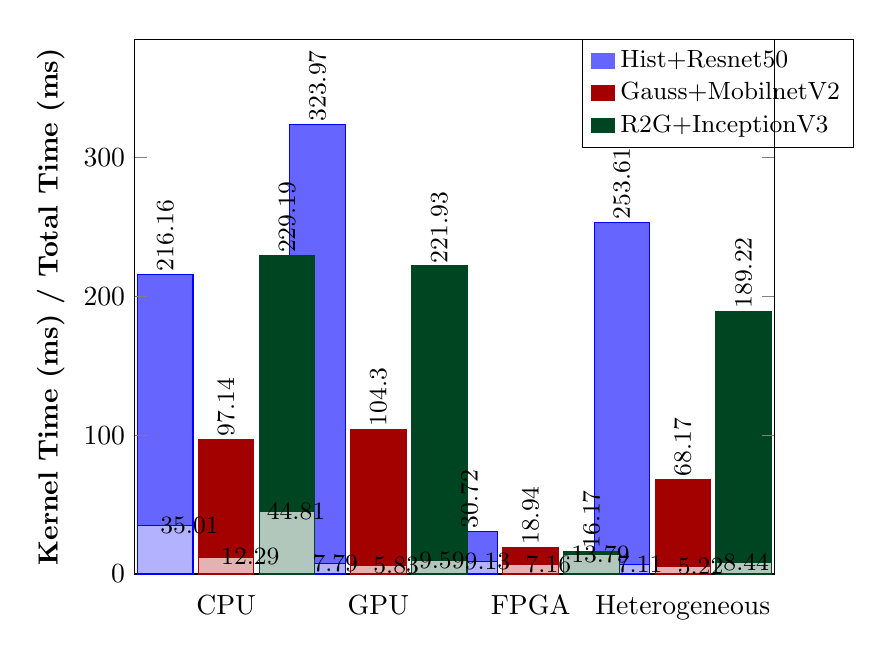
\begin{tikzpicture}
    % Kernel Time Axis
    \begin{axis}[
        width  = 0.8\linewidth,
        major x tick style = transparent,
        ybar,
        ymin=0, ymax=350,
        bar width=20pt,
        enlarge y limits={upper=0.15},
        legend image code/.code={\draw[#1, draw=none] (0cm,-0.1cm) rectangle (0.3cm,0.1cm);},
        ymajorgrids = false,
        ylabel = {\textbf{Kernel Time (ms) / Total Time (ms)}},
        symbolic x coords={CPU,GPU,FPGA,Heterogeneous},
        xtick = data,
        nodes near coords,
        nodes near coords style={font=\small, anchor=west,rotate=90,inner xsep=0.9pt,black},
        scaled y ticks = false,
        enlarge x limits=0.20,
        legend cell align=left,
        legend style={at={(0.7,0.9)},
                       anchor=west,legend columns=1, font=\small},
        axis on top,
    ]
        % Total Time Data Plots
        \addplot[style={blue,fill=blue!60}, every node near coord/.append style={rotate=0, anchor=west,inner xsep=0.9pt}]
            coordinates {(CPU, 216.16) (GPU, 323.97) (FPGA, 30.72) (Heterogeneous, 253.61)}; % Histogram Equalisation + ResNet-50
        \addplot[style={darkcandyapplered,fill=darkcandyapplered}, every node near coord/.append style={rotate=0, anchor=west,inner xsep=0.9pt}]
            coordinates {(CPU, 97.14) (GPU, 104.30) (FPGA, 18.94) (Heterogeneous, 68.17)}; % Gaussian Filter + MobilnetV2
        \addplot[style={forestgreen,fill=forestgreen}, every node near coord/.append style={rotate=0, anchor=west,inner xsep=0.9pt}]
            coordinates {(CPU, 229.19) (GPU, 221.93) (FPGA, 16.17) (Heterogeneous, 189.22)}; % RGB2Gray + InceptionV3
        \legend{Hist+Resnet50, Gauss+MobilnetV2, R2G+InceptionV3}
    \end{axis}

    % Total Time Axis
    \begin{axis}[
        width  = 0.8\linewidth,
        major x tick style = transparent,
        ybar,
        ymin=0, ymax=350,
        bar width=20pt,
        enlarge y limits={upper=0.15},
        legend image code/.code={\draw[#1, draw=none] (0cm,-0.1cm) rectangle (0.3cm,0.1cm);},
        ymajorgrids = false,
        ylabel = {\textbf{}},
        axis y line*=right,
        axis x line=none,
        symbolic x coords={CPU,GPU,FPGA,Heterogeneous},
        xtick = \empty,
        ytick style = {draw=none}, % Hides the y-axis ticks
        yticklabels = {}, % Hides the y-axis labels
        nodes near coords,
        nodes near coords style={font=\small, anchor=west,rotate=0,inner xsep=0.5pt,black,shift={(-2.5pt,0pt)}}, % Adjust shift as needed
        scaled y ticks = false,
        enlarge x limits=0.20,
        legend cell align=left,
        legend style={at={(0.5,1.05)},
                       anchor=west,legend columns=4, font=\small},
    ]
        % Kernel Time Data Plots
        \addplot[style={blue,fill=blue!30}]
            coordinates {(CPU, 35.01) (GPU, 7.79) (FPGA, 9.13) (Heterogeneous, 7.11)}; % Histogram Equalisation + ResNet-50
        \addplot[style={darkcandyapplered,fill=darkcandyapplered!30}]
            coordinates {(CPU, 12.29) (GPU, 5.83) (FPGA, 7.16) (Heterogeneous, 5.22)}; % Gaussian Filter + MobilnetV2
        \addplot[style={forestgreen,fill=forestgreen!30}, every node near coord/.append style={rotate=0, anchor=west,inner xsep=-5pt}]
            coordinates {(CPU, 44.81) (GPU, 9.59) (FPGA, 13.79) (Heterogeneous, 8.44)}; % RGB2Gray + InceptionV3
        % \legend{Hist+Resnet50, Gauss+MobilnetV2, R2G+InceptionV3}
    \end{axis}
\end{tikzpicture}
}  
%     \caption{Kernel and Total Runtime  Comparison of Individual Algorithms and Pipelines on each Hardware Platform. CPU(5900X) GPU(A2000) FPGA(Alveo U50).}
%     \label{fig:HeterogeneousRuntime}
% \end{figure}



\section{CONCLUSION}
\label{sec:conclusion}

In this paper, a scheduler is introduced to partition complex computer vision pipelines, which consist of pre-processing algorithms and convolutional neural networks, namely, \textit{Resnet50}, \textit{Mobilnetv2}, and \textit{InceptionV3}, onto a heterogeneous platform. The scheduler parses image processing code and selects the most suitable accelerator for execution based on a performance cost model or accelerator directives. This model is developed by profiling various imaging algorithms on various accelerators to determine their runtime and energy characteristics. The scheduler leverages PyTorch, ONNX, and TVM to generate computation graphs and produce code targeting GPU and FPGA accelerators. The partitioning and scheduling strategy considers each type of accelerator's unique strengths and weaknesses, optimising for both speed and energy efficiency. 

Experimental results demonstrate the schedulers effectiveness, with the heterogeneous platform consistently outperforming individual accelerators in energy efficiency and runtime across various vision pipelines. On average, the heterogeneous platform achieves significant energy savings, being approximately \(10.11\times\) more efficient than the CPU, \(1.27\times\) more efficient than the FPGA, and \(1.34\times\) more efficient than the GPU. The findings suggest that partitioning and scheduling vision pipelines based on runtime and energy profiles holds the potential for efficient deployment on heterogeneous architectures, offering a viable alternative to GPU/FPGA-only applications. This approach maximises computational resources and significantly reduces energy consumption, making it highly suitable for real-time image processing tasks in resource-constrained environments.


\section{FUTURE WORK}
\label{sec:future work}

Future research will focus on enhancing the scheduling framework for heterogeneous vision systems and optimising task distribution across CPUs, GPUs, and FPGAs using dynamic load balancing and machine learning-based partitioning. This will involve real-time performance metrics and resource availability, leveraging historical data and performance models for informed task allocation. In the scope of convolutional neural network algorithm, layer by layer partitioning on the most optimised processes can be applied to further optimise overall performance of CNN algorithms. To further enhance the efficiency, research will explore integrating emerging technologies such as neural processing units and neuromorphic processors. 

Furthermore, developing a heterogeneity inspired Domain-Specific Language (DSL) for optimising computer vision pipelines will be explored, aiming to provide a higher abstraction and efficient approach to designing and implementing vision algorithms. Domain-specific compilers would be extended to target heterogeneous back-ends with data transfers between accelerators.The scheduler is limited by the manual implementation of direct memory access for each generated code, therefore improvements will involve automatically integrating DMA code, eliminating the bottleneck during the compilation/synthesis process.





\begin{table}
\centering
\setlength{\extrarowheight}{0pt}
\addtolength{\extrarowheight}{\aboverulesep}
\addtolength{\extrarowheight}{\belowrulesep}
\setlength{\aboverulesep}{0pt}
\setlength{\belowrulesep}{0pt}
\caption{Individual Algorithms on various hardware}
\label{tab:hardware_results}
\arrayrulecolor{black}
\resizebox{\linewidth}{!}{%
\begin{tabular}{c|c|c|c|c|c|c|c|c|c|c|c|c} 
\toprule
\rowcolor[rgb]{0.753,0.753,0.753} {\cellcolor[rgb]{0.753,0.753,0.753}} & \multicolumn{3}{c|}{\textbf{Runtime (ms)}} & \multicolumn{3}{c|}{\textbf{Frame per second }} & \multicolumn{3}{c|}{\begin{tabular}[c]{@{}>{\cellcolor[rgb]{0.753,0.753,0.753}}c@{}}\textbf{Energy}\\\textbf{ (Joules)}\end{tabular}} & \multicolumn{3}{c}{\begin{tabular}[c]{@{}>{\cellcolor[rgb]{0.753,0.753,0.753}}c@{}}\textbf{Memory Latency}\\\textbf{(ms)}\end{tabular}} \\ 
\hhline{>{\arrayrulecolor[rgb]{0.753,0.753,0.753}}->{\arrayrulecolor{black}}------------}
\rowcolor[rgb]{0.753,0.753,0.753} \multirow{-2}{*}{{\cellcolor[rgb]{0.753,0.753,0.753}}\textbf{Algorithm }} & \textbf{CPU} & \textbf{GPU} & \textbf{FPGA} & \textbf{CPU} & \textbf{GPU} & \textbf{FPGA} & \textbf{CPU} & \textbf{GPU} & \textbf{FPGA} & \textbf{CPU} & \textbf{GPU} & \textbf{FPGA} \\ 
\midrule
\begin{tabular}[c]{@{}c@{}}Histogram \\Equalisation\end{tabular} &  &  &  &  &  &  & N/A &  &  &  &  &  \\ 
\midrule
Gaussian &  &  &  &  &  &  & N/A &  &  &  &  &  \\ 
\midrule
Resnet18 &  &  &  &  &  &  &  &  &  &  &  &  \\ 
\midrule
Inception  &  &  &  &  &  &  &  &  &  &  &  &  \\
\bottomrule
\end{tabular}
}
\end{table}
\definecolor{Silver}{rgb}{0.752,0.752,0.752}
\begin{table}
\centering
\caption{Results Table of Pipelines on a Heterogeneous Platform. Total Runtime includes device and model initialisation.}
\label{tab:Individualsummary}
\resizebox{\linewidth}{!}{%
\begin{tblr}{
  cells = {c},
  row{1} = {Silver},
  row{2} = {Silver},
  cell{1}{1} = {r=2}{},
  cell{1}{2} = {c=3}{},
  cell{1}{5} = {r=2}{},
  cell{1}{6} = {r=2}{},
  cell{1}{7} = {r=2}{},
  cell{1}{8} = {r=2}{},
  cell{1}{9} = {r=2}{},
  cell{1}{10} = {r=2}{},
  vlines,
  hline{1,3-6} = {-}{},
  hline{2} = {2-4}{},
}
\textbf{Pipeline} & {\textbf{Accelerator for}\\\textbf{ Partitioned Operation}} &  &  & {\textbf{~ Kernel}\\\textbf{Runtime (ms)}} & {\textbf{Kernel Energy}\\\textbf{(Joules)}} & {\textbf{Kernel}\\\textbf{Frames per }\\\textbf{Second} (\textbf{FPS})} & {\textbf{Total }\\\textbf{Runtime}\\\textbf{(ms)}} & {\textbf{Total }\\\textbf{Energy}\\\textbf{(Joules)}\\\textbf{}} & {\textbf{Accuracy}\\\textbf{(\%)}}\\
 & CPU & GPU & FPGA &  &  &  &  &  & \\
{Histogram \\Equalisation \\+ ResNet-50} & x & Resnet-50 & Hist. & 7.11 & 0.27 & 140.65 & 253.61 & 17.75 & 87\\
{Gaussian Filter\\+ MobilnetV2} & x & MobilnetV2 & Gaus. & 5.22 & 0.17 & 191.57 & 68.17 & 4.85 & 82\\
{RGB2Gray\\+ InceptionV3} & x & InceptionV3 & R2G. & 8.44 & 0.035 & 118.48 & 189.22 & 13.24 & 84
\end{tblr}
}
\end{table}
\begin{table}
\centering
\setlength{\extrarowheight}{0pt}
\addtolength{\extrarowheight}{\aboverulesep}
\addtolength{\extrarowheight}{\belowrulesep}
\setlength{\aboverulesep}{0pt}
\setlength{\belowrulesep}{0pt}
\caption{Results Table of Vision Pipelines on Individual Hardware}
\label{tab:heterogenoussummary}
\arrayrulecolor{black}
\resizebox{\linewidth}{!}{%
\begin{tabular}{c|c|l|l|c|l|l|l|l|l|l|l|l} 
\toprule
\rowcolor[rgb]{0.753,0.753,0.753} {\cellcolor[rgb]{0.753,0.753,0.753}} & \multicolumn{3}{c|}{\begin{tabular}[c]{@{}>{\cellcolor[rgb]{0.753,0.753,0.753}}c@{}}\textbf{~ Total }\\\textbf{Runtime (ms)}\end{tabular}} & \multicolumn{3}{c|}{\begin{tabular}[c]{@{}>{\cellcolor[rgb]{0.753,0.753,0.753}}c@{}}\textbf{Total}\\\textbf{Energy usage}\\\textbf{(Joules)}\end{tabular}} & \multicolumn{3}{c|}{\begin{tabular}[c]{@{}>{\cellcolor[rgb]{0.753,0.753,0.753}}c@{}}\textbf{Frames per Second}\\\textbf{(FPS)}\end{tabular}} & \multicolumn{3}{c}{\begin{tabular}[c]{@{}>{\cellcolor[rgb]{0.753,0.753,0.753}}c@{}}\textbf{Memory Latency}\\\textbf{(ms)}\end{tabular}} \\ 
\hhline{>{\arrayrulecolor[rgb]{0.753,0.753,0.753}}->{\arrayrulecolor{black}}------------}
\rowcolor[rgb]{0.851,0.851,0.851} \multirow{-2}{*}{{\cellcolor[rgb]{0.753,0.753,0.753}}\textbf{Pipeline}} & \multicolumn{1}{l|}{\textbf{CPU}} & \textbf{GPU} & \textbf{FPGA} & \multicolumn{1}{l|}{\textbf{CPU}} & \textbf{GPU} & \textbf{FPGA} & \textbf{CPU} & \textbf{GPU} & \textbf{FPGA} & \textbf{CPU} & \textbf{GPU} & \textbf{FPGA} \\ 
\hline
Histogram Equalisation + ResNet-18 & 10.0216 & 2.6381 &  &  & &  & 99.78 & 379.06 & &  & & \\ 
\cmidrule{1-1}\cline{2-13}
 &  &  &  &  &  &  &  &  &  &  &  &  \\ 
\cmidrule{1-1}\cline{2-13}
 &  &  &  &  &  &  &  &  &  &  &  &  \\ 
\cmidrule{1-1}\cline{2-13}
 &  &  &  &  &  &  &  &  &  &  &  &  \\ 
\cmidrule{1-1}\cline{2-13}
 &  &  &  &  &  &  &  &  &  &  &  &  \\
\bottomrule
\end{tabular}
}
\end{table}


\acknowledgments % equivalent to \section*{ACKNOWLEDGMENTS}       
 
This work was partly supported by Newcastle University \& STMicroelectronics Imaging Division.

% References
\bibliography{report} % bibliography data in report.bib
\bibliographystyle{spiebib} % makes bibtex use spiebib.bst

\end{document} 
